Kolejne narzędzie do tworzenia regulatorów i filtrów wejściowych dla
układów o jednym wejściu i jednym wyjściu. Program posiada wygodny interfejs umożliwiający bieżący podgląd charakterystyk czasowych i częstotliwościowych
zarówno układu otwartego (dla regulatora) oraz zamkniętego (obiekt + regulator). Użytkownik definiuje układ poprzez wybór jednego ze schematów, podaje wartości obiektów (np. z Workspace'a), a następnie przechodzi do zakładki poświęconej strojeniu.
Narzędzie uruchamia się poprzez wpisanie komendy

\textit{controlSystemDesigner}.

\begin{figure}[H]
	\centering
	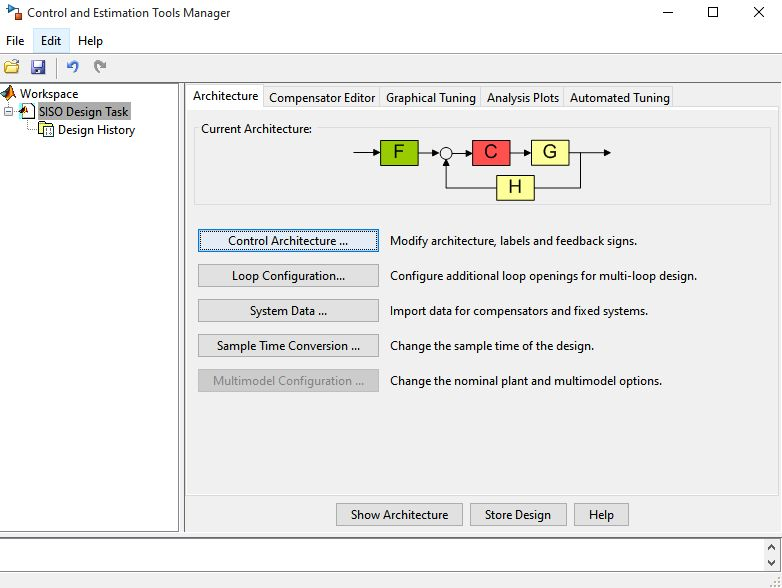
\includegraphics[width=130mm]{SISO_Design_Tool1}
	\caption{Zrzut ekranu przedstawiający narzędzie definiowanie obiektu w SISO Design Tool}
	\label{fig:SISO_Design_Tool1}
\end{figure}
\begin{figure}[H]
	\centering
	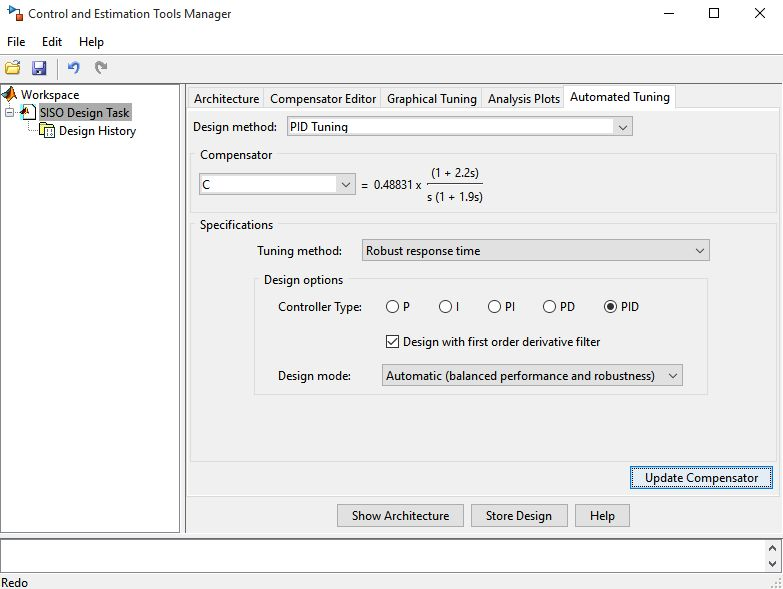
\includegraphics[width=130mm]{SISO_Design_Tool2}
	\caption{Zrzut ekranu przedstawiający proces automatycznego strojenia w SISO Design Tool}
	\label{fig:SISO_Design_Tool2}
\end{figure}



